\documentclass[]{article}
\usepackage{geometry}   % my added package "geometry"
\geometry{letterpaper,tmargin=1in,bmargin=1in,lmargin=2.2cm,rmargin=2.2cm}
\usepackage[colorlinks,bookmarksopen,bookmarksnumbered,
citecolor=green,urlcolor=red]{hyperref}
\hypersetup{pdfauthor={Name}}
%%%%%%%%%%%%%%%%%%%%%%%%%%%%%%%%%%%%%%%%%%%%%%%%%%%%%%%%%%%%%%%%%%%%%%%%%
%\usepackage{graphicx}
\usepackage{graphics}
\usepackage{epsfig}
\usepackage{epstopdf}
\usepackage{amsfonts}
\usepackage{amssymb}
\usepackage{booktabs}
\usepackage{color,soul}
%%%%%%%%%%%%%%%%%%%%%%%%%%%%%%%%%%%%%%%%%%%%%%%%%%%%%%%%%%%%%%%%%
\usepackage{amsmath}
\usepackage{cleveref}
\usepackage{authblk}
%\usepackage[fleqn]{amsmath}
\usepackage{lineno}
\usepackage{tikz}
\usepackage{standalone}
\usetikzlibrary{calc,patterns,arrows.meta,shapes.arrows,intersections,positioning}
\usetikzlibrary{decorations.pathmorphing,backgrounds,fit,petri}
\usepackage[percent]{overpic}
%%%%%%%%%%%%%%%%%%%%%%%%%%%%%%%%%%%%%%%%%%%%%%%%%%%%%%%%%%%%%%%%%
\usepackage{xcolor}
\usepackage{listings}
\lstset { %
	language=C++,
	backgroundcolor=\color{blue!5}, % set backgroundcolor
	basicstyle=\footnotesize\color{black},% basic font settingbasicstyle=\ttfamily\color{black}
	keywordstyle=\color{red},
	commentstyle=\color{violet},
	stringstyle=\color{blue},
	xleftmargin=2em,
	frame=single,
	framexleftmargin=2em,
	numbers=left,
	numberstyle=\tiny,
	numbersep=8pt,
}
%%%%%%%%%%%%%%%%%%%%%%%%%%%%%%%%%%%%%%%%%%%%%%%%%%%%%%%%%%%%%%%%%
\renewcommand\thesubsection{\thesection\Alph{subsection}}
%%%%%%%%%%%%%%%%%%%%%%%%%%%%%%%%%%%%%%%%%%%%%%%%%%%%%%%%%%%%%%%%%
\renewcommand\lstlistingname{Header}
\renewcommand\lstlistlistingname{Header}
%%%%%%%%%%%%%%%%%%%%%%%%%%%%%%%%%%%%%%%%%%%%%%%%%%%%%%%%%%%%%%%%%%%%
%opening
\begin{document}
\title{HiperLife Tutorial: Poisson Equation}
\author{Arash Imani\thanks{Disclaimer: The implemented code (as can be seen in its respective section) is a part of HiperLife primary tutorials, so it is programmed by others.}}
\affil{LaCàN}
\maketitle

\linenumbers
\section{Problem Definition} \label{sec: pd}
The Poisson equation extends from the simpler Laplace equation, which assumes no sources. When sources are present, the Poisson equation becomes useful in describing how fields, such as electric or gravitational potential fields, are influenced by these sources. The Poisson equation appears frequently in classical physics and underlies much of the theoretical framework for modeling potential fields such as Electrostatics, Gravitational Potential, Heat Conduction and Fluid Mechanics.The Poisson equation's versatility comes from its ability to connect a spatially varying source (charge, mass, heat, etc.) with a field (potential, temperature, pressure, etc.) that responds to that source. Solving the Poisson equation in any given physical context allows scientists and engineers to predict how a system will respond to internal sources, like an electric charge distribution or a temperature source, and adjust designs accordingly.
\begin{figure}[htbp]
	\centering
	
\documentclass[preprint,12pt,a4]{standalone}
\usepackage{geometry}   % my added package "geometry"
\geometry{letterpaper,tmargin=1in,bmargin=1in,lmargin=2.5cm,rmargin=2.5cm}
\usepackage{tikz}
\usetikzlibrary{calc,patterns,arrows.meta,shapes.arrows,intersections,positioning}
\usetikzlibrary{decorations.pathmorphing,backgrounds,fit,petri}
\usepackage{standalone}
\begin{document}
	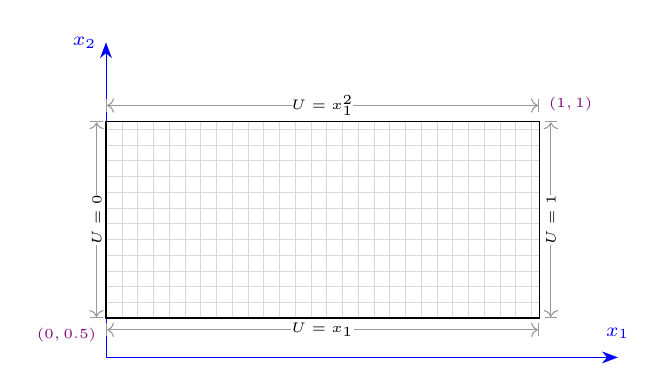
\begin{tikzpicture} [{place/.style={rectangle,draw=blue!50,fill=blue!20,ultra thin,inner sep=0.8mm}},{place2/.style={circle,draw=black!50,ultra thin,inner sep=0.8mm}},{linest/.style={color=gray,ultra thin}}]
	%%coordinates of corners of Beam
	\coordinate (A) at (0.0,0.0);
	\coordinate (B) at (5.5,0.0);
	\coordinate (D) at ($(A)+(0.0,2.5)$);
	\coordinate (C) at ($(B)+(D)$);
	%%axes
	\draw [{Stealth[length=2mm]}-{Stealth[length=2mm]}, help lines,blue] ($(B)+(1,-0.5)$) -- (0,-0.5) -- ($(D)+(0,1)$);
	\node [below,color = blue,font=\scriptsize] at ($(B)+(1,0)$) {$x_1$};
	\node [left,color = blue,font=\scriptsize] at ($(D)+(0,1)$) {$x_2$};
	%%fixed boundary
	%\draw [pattern = crosshatch] ($(A)-(0.1,0.3)$) rectangle ($(D)+(0.0,0.3)$);
	%%mesh
	\draw [line width=0.1pt,gray!30,step=2mm](A) grid (C);
	%%Beam	
	\draw [color=black](A)node[font=\tiny, violet,below left]{$(0,0.5)$} -- (B) -- (C) node[font=\tiny, violet,above right]{$(1,1)$} -- (D) -- cycle;
	%%Concentrate Force Vector
	%\draw [-{Latex[length=2mm]},color=purple, thick] ($(C)+(0.0,1.0)$) -- (C);
	%\node[above,color=purple] at ($(C)+(0.0,1.0)$) {$P$};
	%%B.C
	\draw [|<->|,gray!80]($(A)+(0,-0.15)$) --($(B)+(0,-0.15)$) node[fill=white,midway,inner sep=0.1pt, font=\tiny,text=black] {$U=x_{1}$};
	\draw [|<->|,gray!80]($(B)+(0.15,0.0)$)--($(C)+(0.15,0.0)$) node [fill=white,midway, sloped, font=\tiny, inner sep=0.05pt, text=black] {$U=1$};
	
	\draw [|<->|,gray!80]($(C)+(0,0.2)$) --($(D)+(0,0.2)$) node[fill=white,midway,inner sep=0.01pt, font=\tiny,text=black] {$U=x_{1}^2$};
	\draw [|<->|,gray!80]($(A)+(-0.12,0.0)$)--($(D)+(-0.12,0.0)$) node [fill=white,midway,sloped, font=\tiny, inner sep=0.05pt, text=black] {$U=0$};
	\end{tikzpicture}
\end{document}
	\caption{Geometry, BC and computational domain used for the analysis of Poisson problem.}
	\label{fig_SB}
\end{figure}

In practical applications, boundary conditions are often applied to solve the Poisson equation in specific regions, which is essential for real-world systems that are typically bounded by physical surfaces. The equation is solved using methods such as separation of variables, Green's functions, or numerical techniques like finite difference or finite element methods, especially in complex geometries.
\section{Governing Equations} \label{sec: ge}
Poisson Equation is a simple elliptic model, given by
\begin{equation}\label{eq1}
	\begin{aligned}
		-\Delta U = -\nabla^2 U = -\frac{\partial^2 U}{\partial x_{1}^2} - 
		\frac{\partial^2 U}{\partial x_{2}^2}=f
	\end{aligned}
\end{equation}
We will use this equation in this example for introducing the implemention of finite
element method in the HiperLife. Notice that here we have used $f = 0$. As shown in Figure \ref{fig_SB}, We have used homogeneous Dirichlet ($U=0 ,\quad U=1$) along the lines ($x_{1}=0,\quad x_{1}=1$), and along the lines ($x_{2}=0.5,\quad x_{2}=1$) we applied Inhomogenous Dirichelet ($U=x_{1} ,\quad U=x_{1}^2$), respectively.
\section{Weak Form} \label{sec: wf}
The starting point for the development of the finite element model of Eq. (\ref{eq1}) is its weak form.
The variational formulation of our model problem reads: Find $u \in V$ such that
\begin{equation}\label{eq2}
	\begin{aligned}
		\mathcal{F}(u;v) = 0 \quad \forall v \in \hat{V}
	\end{aligned}
\end{equation}
where
\begin{equation}\label{eq3}
	\begin{aligned}
		\mathcal{F}(u; v) =-\int_\Omega v \nabla \cdot \nabla u - v f \mathrm{d}\Omega\thinspace .
	\end{aligned}
\end{equation}
and
\begin{equation}\label{eq4}
	\begin{aligned}
		\hat{V} &= \{v \in H^1(\Omega) : v = 0 \text{ on } \partial \Omega\}, \\
		V &= \{v \in H^1(\Omega) : v = 0 \text{ on } x_1=0, \ v = 1\text{ on }x_1=1, \ v= x_1 \text{ on } x_2=0.5, \ v= x_1^2 \text{ on } x_2=1\}\thinspace.
	\end{aligned}
\end{equation}
where $v$ is a test function, which will be equated, in the our FE model to the interpolation function used for $u$.The discrete problem arises as usual by restricting $V$ and $\hat{V}$ to a pair of discrete spaces. using integrating by part this expression over $\Omega$, we have
\begin{equation}\label{eq5}
	\begin{aligned}[b]
		\mathcal{F}(u; v)=-\int_\Omega \nabla \cdot [v \nabla u] \ \mathrm{d} \Omega + \int_\Omega  \nabla v \nabla u \ \mathrm{d} \Omega - \int_\Omega vf \ \mathrm{d} \Omega\thinspace .
	\end{aligned}
\end{equation}
Using Gauss’s theorem we get
\begin{equation}\label{eq6}
	\begin{aligned}[b]
		\mathcal{F}(u; v)=-\int_\Gamma [v \nabla u] \cdot \mathbf{n} \ \mathrm{d} \Gamma + \int_\Omega  \nabla v \nabla u \ \mathrm{d} \Omega - \int_\Omega vf \ \mathrm{d} \Omega\thinspace.
	\end{aligned}
\end{equation}
By applying boundary condition since we do not have any flux, the final relation of weak form would be as
\begin{equation}\label{eq7}
	\begin{aligned}[b]
		\mathcal{F}(u; v)=\int_\Omega  \nabla v \nabla u \ \mathrm{d} \Omega - \int_\Omega vf \ \mathrm{d} \Omega\thinspace.
	\end{aligned}
\end{equation}
\section{Finite Element Model} \label{sec: fem}
For Ritz-Galerkin FE model, the choice of the test functions is restricted to the spaces of approximation functions used for the solution field. Suppose that the variable $u$ approximated by expansions of the form
\begin{equation}\label{eq8}
	\begin{aligned}
		u(\mathbf{x})= \sum_{j=1}^{M} \phi_j(\mathrm{x}) u_j = \boldsymbol{\Phi}^T\mathbf{u} \thinspace.
	\end{aligned}
\end{equation}
By substituting Eq. (\ref{eq8}) in Eq. (\ref{eq7}) we get
\begin{equation}\label{eq9}
	\begin{aligned}[b]
		\mathcal{F}(u; \phi)=\int_\Omega  \nabla \phi_i \nabla \phi_j u_j\ \mathrm{d} \Omega - \int_\Omega \phi_i f_i \ \mathrm{d} \Omega\thinspace.
	\end{aligned}
\end{equation}
The above equations can be written symbolically in matrix form as
\begin{equation}\label{eq10}
	\begin{aligned}
		\mathbf{K}\mathbf{u} = \mathbf{F}\thinspace.
	\end{aligned}
\end{equation}
The coefficient matrices $\mathbf{K}$ and $\mathbf{F}$ shown in Eq. (\ref{eq15}) are defined as
\begin{equation}\label{eq11}
	\begin{aligned}[b]
		K(i,j) &= \int_{\Omega_{T}} (\frac{\partial \phi_{i}}{\partial x_{1}}
		\frac{\partial \phi_{j}}{\partial x_{1}}+\frac{\partial \phi_{i}}{\partial x_{2}} 
		\frac{\partial \phi_{j}}{\partial x_{2}}) dA\\
		F(i) &= \int_{\Omega_{T}} \phi_{i}f_i \mathrm{d}A
	\end{aligned}
\end{equation}
keep in mind that in our case $f=0$, too. Note that $\mathrm{d}A=\mathrm{d}x_{1} \times \mathrm{d}x_{2}=jac\mathrm{d}\xi \mathrm{d}\eta$, which $jac=\mathrm{det}(Jacobian)$\footnote{for more details see the Appendix}. The elemental representation of the vector and matrix required for implementation in the Hiperlife would have the format of 
\begin{equation}\label{eq12}
	\begin{aligned}[b]
		Ak(i,j) &= jac \times \left[\frac{\partial \phi_{i}}{\partial x_{1}}
		\frac{\partial \phi_{j}}{\partial x_{1}}+\frac{\partial \phi_{i}}{\partial x_{2}} \frac{\partial \phi_{j}}{\partial x_{2}}\right], \\
		Bk(i) &= jac \times [\phi_{i}f]\thinspace .
	\end{aligned}
\end{equation}
\section{Choice of Elements} \label{sec: coe}
Thus, for this simple problem every Lagrange and serendipity family of interpolation functions are admissible for the interpolation of the temperature field, our choice is would be linear quadrilateral element.Linear  Quadrilateral Elements is the simplest quadrilateral element consists of four nodes. The associated interpolation functions for geometry and field variables are bilinear.
\begin{equation}\label{eq13}
	\begin{aligned}[b]
		\boldsymbol{\Phi}_{I}(\xi, \eta) = \frac{1}{4}(1+\xi_I\xi)(1+\eta_I\eta) \quad (I \ \text{from} \ 1 \ \text{to} \ 4)
	\end{aligned}
\end{equation}

where $\xi_{I}$ and $\eta_{I}$ are the corner coordinates at element $T$ in domain of $\Omega_{T} \in (-1,1)^2$. As it shown in Figure \ref{fig_elm} we are using $2 \times 2$ Gauss–Legendre quadrature integration.
\begin{figure}[htbp]
	\centering
	\input{Figures/element2.tex}
	\caption{Linear quadrilateral element used for finite element model.}
	\label{fig_elm}
\end{figure}

In this example each node only have one degree of freedom and for the purpose of discretization we use $500 \times 500$ uniform mesh.
\begin{figure}[htbp]
	\centering
	\input{Figures/flowchart.tex}
	\caption{Flow chart.}
	\label{fig_flw}
\end{figure}
\section{Implementation} \label{sec: imp}
In this section, we present the implementation of our solution in the Hiperlife. The program is divided into three separate files, main part which we create our problem by the Hiperlife headers, auxiliary header where we introduce parameters and declare defined functions, and at last auxiliary file, where we define some functions which provide required matrices like the tangent matrix. As it is already mentioned this code is from the Hiperlife primary tutorials and for any use the Copyright policy and License should be check from the project homepage\footnote{ https://hiperlife.gitlab.io/hiperlife}. The Flowchart of a typical HiperLife program is shown in Figure \ref{fig_flw}.
 
\subsubsection{Poisson.cpp} \label{sec: m.cpp}
\nolinenumbers
\begin{lstlisting}
/*
*******************************************************************************
Copyright (c) 2017-2023 Team hiperlife
Authors: Daniel Santos-OlivAn, Alejandro Torres-SAnchez and Guillermo Vilanova
Contributors:
*******************************************************************************
This file is part of hiperlife
Project homepage: https://hiperlife.gitlab.io/hiperlife
Distributed under the GNU General Public License, see the accompanying
file LICENSE or https://opensource.org/license/gpl-3-0.
*******************************************************************************
*/



// hiperlife headers
#include "hl_Core.h"
#include "hl_ParamStructure.h"
#include "hl_Parser.h"
#include "hl_TypeDefs.h"
#include "hl_GlobalBasisFunctions.h" 
#include "hl_StructMeshGenerator.h"
#include "hl_MeshLoader.h"
#include "hl_DistributedMesh.h"
#include "hl_FillStructure.h"
#include "hl_DOFsHandler.h"
#include "hl_HiPerProblem.h"
#include "hl_LinearSolver_Iterative_AztecOO.h"
#include "hl_LinearSolver_Direct_MUMPS.h"

//using another header file for filling the elemental linear  
#include "AuxPoisson.h"

int main(int argc, char** argv)
{
	using namespace std;
	using namespace hiperlife;
		
	// **************************************************************//
	// *****                 INITIALIZATION                     *****//
	// **************************************************************//
	hiperlife::Init(argc, argv);
	SmartPtr<ParamStructure> paramStr = CreateParamStructure<PoissonParams>();
	// **************************************************************//
	// *****                   MESH CREATION                    *****//
	// **************************************************************//
	//====================== Mesh generation ======================//
	
	SmartPtr<StructMeshGenerator> structMesh = Create<StructMeshGenerator>();
	structMesh->setNDim(3);
	structMesh->setBasisFuncType(BasisFuncType::Lagrangian);
	structMesh->setBasisFuncOrder(1);
	structMesh->setElemType(ElemType::Square);
	structMesh->genRectangle(500, 500, 1.0, 0.5);
	structMesh->translateY(0.5);
	//===========             Distribute mesh            ===========//
	SmartPtr<DistributedMesh> disMesh = Create<DistributedMesh>();
	disMesh->setMesh(structMesh);
	disMesh->setBalanceMesh(true);
	disMesh->Update();
	
	// **************************************************************//
	// *****               DOFsHANDLER CREATION                 *****//
	// **************************************************************//
	
	//===========           Create DOFHandler            ===========//
	SmartPtr<DOFsHandler> dofHand = Create<DOFsHandler>(disMesh);
	dofHand->setNameTag("dofHand");
	dofHand->setNumDOFs(1);
	dofHand->Update();
	//===========          Boundary conditions          ===========//
	dofHand->setBoundaryCondition(0, 0.0);
	dofHand->setBoundaryCondition(0, MAxis::Xmax, 1.0);
	dofHand->setBoundaryCondition(0, MAxis::Ymin, [](double x){return x;});
	dofHand->setBoundaryCondition(0, MAxis::Ymax, [](double x){return x*x;});
	dofHand->UpdateGhosts();
	
	
	// **************************************************************//
	// *****               HIPERPROBLEM CREATION                *****//
	// **************************************************************//
	SmartPtr<HiPerProblem> hiperProbl = Create<HiPerProblem>();
	hiperProbl->setParameterStructure(paramStr);
	hiperProbl->setDOFsHandlers({dofHand});
	
	//===========            Set integration             ===========//
	hiperProbl->setIntegration("Integ", {"dofHand"});
	hiperProbl->setCubatureGauss("Integ", 3);
	hiperProbl->setElementFillings("Integ", ElementFilling);
	
	//===========                 Update                ===========//
	hiperProbl->Update();
	
	//===========               Set solver               ===========//
	
	SmartPtr<MUMPSDirectLinearSolver> solver = Create<MUMPSDirectLinearSolver>();
	solver->setHiPerProblem(hiperProbl);
	solver->setVerbosity(MUMPSDirectLinearSolver::Verbosity::Extreme);
	solver->setDefaultParameters();
	solver->Update();
	
	solver->solve();
	hiperProbl->UpdateSolution();
	
	// The results
	dofHand->printFileLegacyVtk("Poisson");
	// for visualization purposes.
	ofstream rhsFile;
	rhsFile.open(paramStr->getStringParameter(PoissonParams::filemesh)
	+to_string(dofHand->myRank())+".txt");
	hiperProbl->sol->Print(rhsFile);
	rhsFile.close();
	
	
	// **************************************************************//
	// *****                    FINALIZE                        *****//
	// **************************************************************//
	
	hiperlife::Finalize();
	return 0;
}

\end{lstlisting}
\subsubsection{AuxPoisson.h} \label{sec: a.h}
\begin{lstlisting}
/*
*******************************************************************************
Copyright (c) 2017-2023 Team hiperlife
Authors: Daniel Santos-Olivan, Alejandro Torres-Sanchez and Guillermo Vilanova
Contributors:
*******************************************************************************
This file is part of hiperlife
Project homepage: https://hiperlife.gitlab.io/hiperlife
Distributed under the GNU General Public License, see the accompanying
file LICENSE or https://opensource.org/license/gpl-3-0.
*******************************************************************************
*/


#ifndef AUXPoisson_H
#define AUXPoisson_H

// C headers
#include <iostream>

// hiperlife headers
#include "hl_ParamStructure.h"
#include "hl_FillStructure.h"
#include "hl_DOFsHandler.h"
#include "hl_HiPerProblem.h"

struct PoissonParams
{
	enum RealParameters
	{
		force
	};
	enum StringParameters
	{
		filemesh
	};
	HL_PARAMETER_LIST DefaultValues
	{
		{"force", 0.0},
		{"filemesh", ""},
	};
};


void ElementFilling(hiperlife::FillStructure& fillStr);

#endif
\end{lstlisting}
\subsubsection{AuxPoisson.cpp} \label{sec: a.cpp}
\begin{lstlisting}
// hiperlife headers
#include "hl_Core.h"
#include "hl_ParamStructure.h"
#include "hl_Parser.h"
#include "hl_TypeDefs.h"
#include "hl_GlobalBasisFunctions.h"
#include "hl_StructMeshGenerator.h"
#include "hl_DistributedMesh.h"
#include "hl_FillStructure.h"
#include "hl_DOFsHandler.h"
#include "hl_HiPerProblem.h"
#include "hl_LinearSolver_Iterative_AztecOO.h"
#include "hl_LinearSolver_Direct_MUMPS.h"
#include "AuxPoisson.h"

void ElementFilling(hiperlife::FillStructure& fillStr)
{
	using namespace std;
	using namespace hiperlife;
	using namespace hiperlife::Tensor;
	
	//===========          Initialize variables           ==========//
	SubFillStructure& subFill = fillStr["dofHand"];
	//   which we use to declare the variables:
	int eNN  = subFill.eNN;       // Number of neighbor nodes
	int pDim = subFill.pDim;      // Number of parametric dimension
	wrapper<double,1>  bf(subFill.nborBFs(), eNN);;
	tensor<double,2> Dbf_g(eNN,pDim);    //[dN_i/dx_1 dN_i/dx_2]
	double jac; //Jacobian (differential of line/area/volume)
	GlobalBasisFunctions::gradients(Dbf_g, jac, subFill);
	
	
	// We are going to fill the matrix and the right hand side. Here, we define
	//   the matrix Ak (eNN*eNN) and the vector Bk (eNN).
	wrapper<double,2> Ak(fillStr.Ak(0, 0).data(),eNN,eNN);
	wrapper<double,1> Bk(fillStr.Bk(0).data(),eNN);
	
	//=====================  Fill linear system =====================//
	//
	// We loop through the neighboring nodes to fill both the matrix
	//    and the right-hand side at the same time
	
	// Fill matrix
	//Ak = jac * Dbf_g * Dbf_g.T();
	// Fill RH
	//Bk = jac * bf * force;
	
	//using ttl::index::i, ttl::index::j, ttl::index::a;
	// Fill matrix
	//Ak = (jac * Dbf_g(i,a) * Dbf_g(j,a))(i,j);
	// Fill RH
	//Bk = (jac * bf(i) * force)(i);
	
	for (int i = 0; i < eNN; i++)
	{
		for (int j = 0; j < eNN; j++)
		{
			// Compute the product of the gradient of the basis functions
			double dotij{};
			for (int d = 0; d < pDim; d++)
			dotij += Dbf_g(i,d)*Dbf_g(j,d);
			
			// Fill matrix
			Ak(i,j) += jac * dotij;
		}
		
		// Fill RHS
		Bk(i) += jac * bf(i) * force;
	}
	
}
\end{lstlisting}
\section{Results} \label{sec: rst}
In this section, we present the results of our solution. The contour demonstration of result $u$ is also shown in Figure \ref{fig_rst}.
\begin{figure}[htbp]
	\centering
	\includegraphics[width=0.6\textwidth]{Figures/result.png}
	\caption{Solution.}
	\label{fig_rst}
\end{figure}

\pagebreak
\section*{Appendix} \label{sec: apx}
In this section we present the derivation behind hiperlife function that calculates the gradients of basis functions and Jacobian.
by the linear mapping between $(\xi,\eta)$ and $(x_{1},x_2)$, we can define $\frac{\partial \phi}{\partial x_{1}}$ and $\frac{\partial \phi}{\partial x_{2}}$
\begin{equation}\label{eq14}
	\begin{aligned}[b]
		&
		\frac{\partial \phi}{\partial \xi} = \frac{\partial \phi}{\partial x_{1}}\frac{\partial x_{1}}{\partial \xi}+\frac{\partial \phi}{\partial x_{2}}\frac{\partial x_{2}}{\partial \eta}\\
		& 
		\frac{\partial \phi}{\partial \eta} = \frac{\partial \phi}{\partial x_{1}}\frac{\partial x_{1}}{\partial \xi}+\frac{\partial \phi}{\partial x_{2}}\frac{\partial x_{2}}{\partial \eta}
	\end{aligned}
\end{equation}
Since $x=x(\xi,\eta)$, we get

\begin{equation}\label{eq15}
	\begin{aligned}[b]
		\begin{bmatrix}
			dx_{1}\\
			\\
			dx_{2}  
		\end{bmatrix}
		= \begin{bmatrix}
			\frac{\partial x_{1}}{\partial \xi}       & \frac{\partial x_{2}}{\partial \xi} \\
			\\
			\frac{\partial x_{1}}{\partial \eta}       &\frac{\partial x_{2}}{\partial \eta}\\
		\end{bmatrix}
		\begin{bmatrix}
			d \xi\\
			\\
			d \eta
		\end{bmatrix}
	\end{aligned}
\end{equation}
%
by defining Jacobian as
\begin{equation}\label{eq16}
	\begin{aligned}[b]
		J = \begin{bmatrix}
			\frac{\partial x_{1}}{\partial \xi}       & \frac{\partial x_{2}}{\partial \xi} \\
			\\
			\frac{\partial x_{1}}{\partial \eta}       &\frac{\partial x_{2}}{\partial \eta}\\
		\end{bmatrix}
	\end{aligned}
\end{equation}
so we can rewrite the Eq. (\ref{eq14}) as

\begin{equation}\label{eq17}
	\begin{aligned}[b]
		\begin{bmatrix}
			\frac{\partial \phi}{\partial x_{1}}\\
			\\
			\frac{\partial \phi}{\partial x_{2}}  
		\end{bmatrix}
		= J^{-1}
		\begin{bmatrix}
			\frac{\partial \phi}{\partial \xi}\\
			\\
			\frac{\partial \phi}{\partial \eta}
		\end{bmatrix}
	\end{aligned}
\end{equation}
where $J^{-1}$ is
\begin{equation}\label{eq18}
	\begin{aligned}[b]
		J^{-1} = \frac{1}{\mathrm{det}J}\begin{bmatrix}
			 \frac{\partial x_{2}}{\partial \eta}    & -\frac{\partial x_{2}}{\partial \xi} \\
			\\
			-\frac{\partial x_{1}}{\partial \eta}      &\frac{\partial x_{1}}{\partial \xi}\\
		\end{bmatrix}
	\end{aligned}
\end{equation}
so by the known relation for basis functions like Eq. (\ref{eq13}), one can calculate the jacobian and the gradient of basis function.
\end{document}
